\chapter{Introduction}
\label{chapter:intro}

\pagenumbering{arabic}

In the past few years, algorithms of computer vision and especially artificial intelligence and deep neural networks brought promising results in image data processing, mostly in the tasks of object detection, semantic segmentation, and classification \cite{LeCun2015}. These advancements may have a significant impact in a vast number of fields, one of them being medicine \cite{Hu2023, He2023, Wemmert2021}. 

In medicine, different types of imaging techniques are being used to provide both non-invasive and invasive visualizations of internal organs, tissues, and other structures. Among non-invasive techniques, we can count, for example, X-ray radiography, ultrasound imaging, magnetic resonance imaging (MRI), and computed tomography (CT). Apart from them, we also mentioned invasive techniques - these are necessary when doctors need to examine a microscopic piece of tissue, e.g., potential tumor tissue or tissue that is known to be a tumor. This is a discipline called histology or histopathology. Doctors can obtain the tissue either by performing a biopsy or surgical resection. Biopsy is a less invasive method - it involves inserting a needle into the patient's body tissue and taking out a small sample. On the other hand, surgical resection is much more invasive and involves some sort of surgical procedure during which the desired piece of tissue is removed. Depending on what doctors want to examine, these samples are then processed further. In the histopathology domain, staining of these images with chemicals is a common practice. This staining helps to create visual contrast between cells, tissues, and other objects on the image slide. Hematoxylin and eosin staining (H\&E staining) is the most widely used staining method for histopathology slides \cite{Dey2022}. Both its components are used to stain different regions of the image. Hematoxylin is responsible for colorizing cell nuclei into shades of deep blue and purple, while eosin is used for staining the extracellular matrix, cytoplasm, and connective tissues in shades of pale red and pink \cite{Dey2022}. An example of this staining on a histopathology image can be seen in Figure \ref{fig:h&e-image}.

\begin{figure}[h]
\begin{centering}
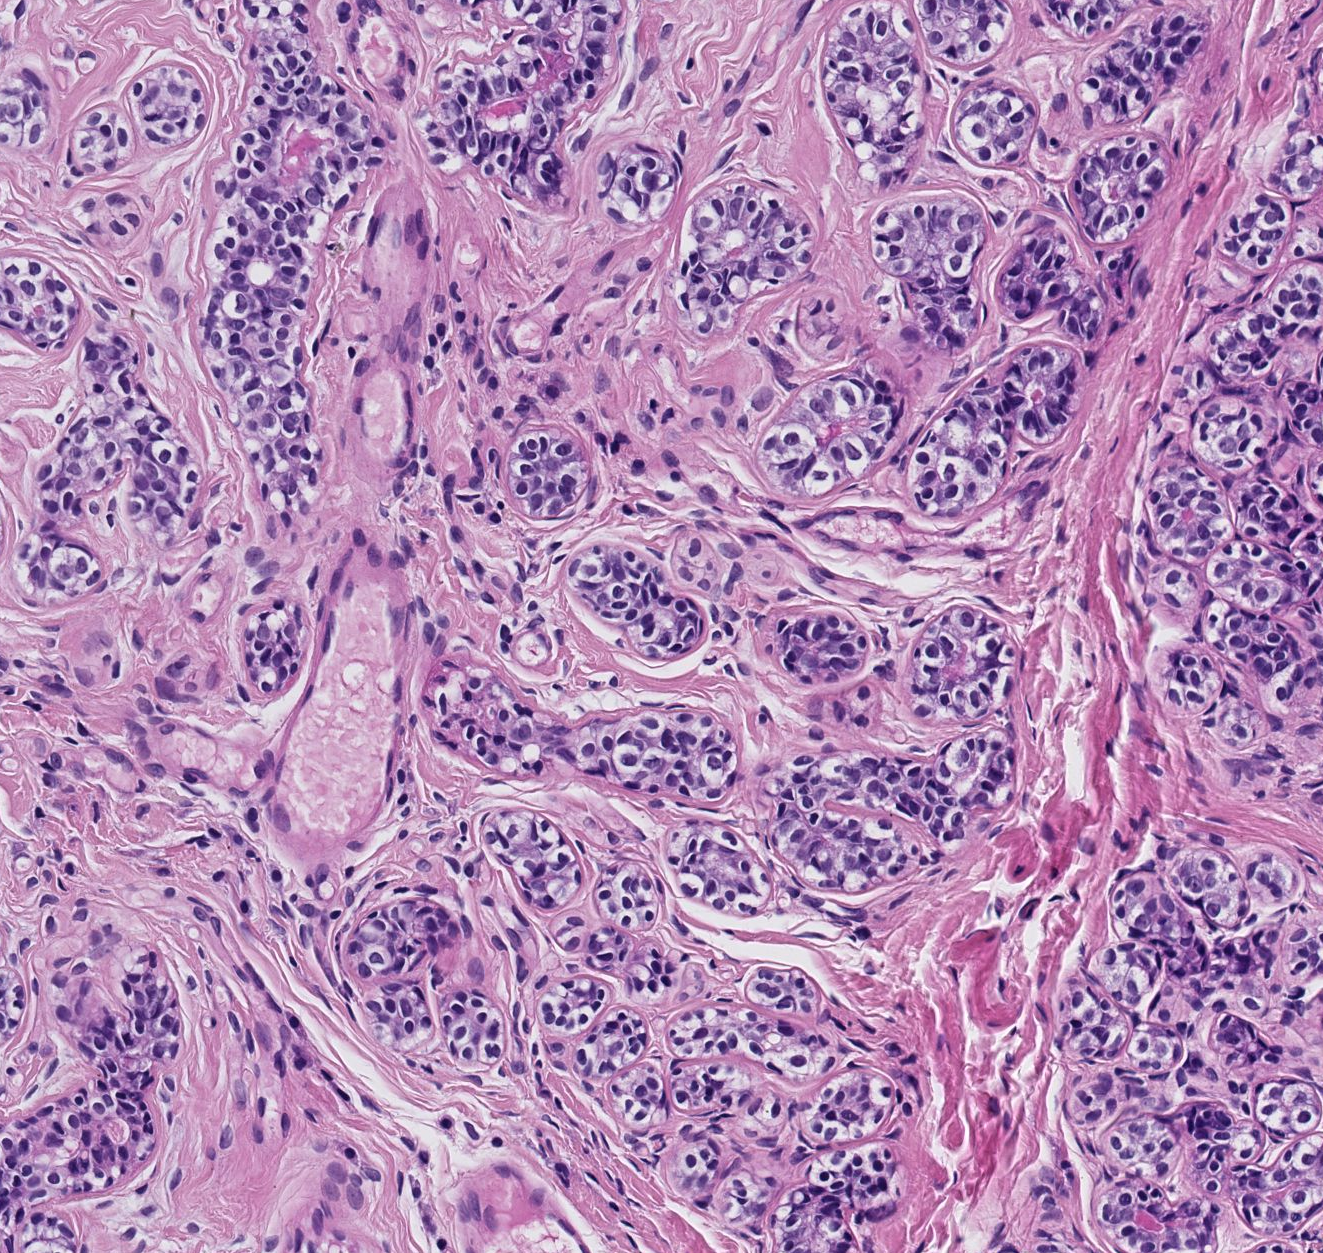
\includegraphics[width=8cm]{assets/images/histology_image_example.png}
\par\end{centering}
\caption{Example of histology image stained with hematoxylin and eosin \label{fig:h&e-image}}
\end{figure}

Slides stained by these chemicals are then examined by histopathology experts who try to identify key features that would determine a diagnosis, future treatment plan, or other subsequent steps. A very good example of this whole process can serve as a method of adjusting treatment for patients who suffer from breast cancer.

\section{Motivation}

In recent decades, breast cancer has been one of the leading causes of death among women and the second most commonly diagnosed type of cancer worldwide \cite{Bray2024, Siegel2023}. According to \cite{Bray2024} in 2022, breast cancer was attributed to approximately 2.3 million newly diagnosed patients - this represents 11.6\% of all diagnosed cancer patients in that year and 666,000 deaths, comprising 6.9\% of all cancer deaths. \cite{Siegel2023} informs that in the USA in the year of 2023, breast cancer among women accounted for more than 297,000 new cases - 31\% of all new female cancer cases and more than 43,000 deaths - 15\% of all female cancer deaths.

When dealing with breast cancer, one needs to keep in mind that there are also different subtypes of breast cancer. Firstly introduced in \cite{Perou2000}, we now know four breast cancer molecular subtypes, based on the positivity or negativity of several receptors. These receptors are Human Epidermal Growth Factor Receptor 2 (HER2) and Hormonal Receptor (HR), which are positive if either Estrogen or Progesterone receptors are positive; otherwise, it is negative. These four classes, along with respective receptor statuses, can be seen in Table \ref{tab:breast_cancer_subtypes}.

\begin{table}[H]
 \centering
 \caption{Breast Cancer Molecular Subtypes and Receptor Statuses}
 \label{tab:breast_cancer_subtypes}
 \begin{tabular}{|l|c|c|c|}
 \hline
 \textbf{Subtype Class} & \textbf{Hormone Receptor (HR)} & \textbf{HER2} \\
 \hline
 Luminal A & Positive & Negative \\
 \hline
 Luminal B & Positive & Positive \\
 \hline
 HER2-enriched & Negative & Positive \\
 \hline
 Triple Negative (TNBC) & Negative & Negative \\
 \hline
 \end{tabular}
\end{table}

From the aforementioned subtypes, the last three are the ones that currently have the worst prognosis \cite{Schalper2022, Zhang2024}. Identifying and using certain biomarkers could potentially improve the prognosis of patients with these subtypes of breast cancer. Tumor-infiltrating lymphocytes (TILs) appear as such biomarkers, especially their presence, number, and spatial organization within the tumor and tumor-related tissue \cite{Salgado2015, Denkert2018, Amgad2019}. However, manual identification and visual recognition of TILs from H\&E-stained slides is a difficult, time-consuming, and error-prone task even when performed by experienced histopathology experts \cite{Salgado2015, Amgad2019}.

\section{Objectives}
Manual analysis of histopathology slides is expensive, takes a long time to complete, and requires highly trained professionals and quality assurance by performing peer reviews \cite{Wemmert2021}. With the invention of virtual microscopy, which enables H\&E-stained glass slides to be converted into digital slides, and the introduction of Whole-slide Images (WSIs), the field is entering a new era. The term Digital Pathology or Digital Histopathology is often used. In Digital Pathology, much effort is put into developing tools that would help medical experts to semi- or fully automate the visual analysis of the digital slides. Entities such as different tissue types and cells can be identified and classified.

Deep learning has shown extreme potential in many areas, including medicine and processing of medical image data \cite{LeCun2015}. The usage of deep learning models also introduces a new challenge: for them to produce reasonably good results, they need a huge amount of high-quality data \cite{Santosh2022-3}. Precise manual annotation of histology slides is not an easy nor a cheap task, as we have mentioned earlier. Therefore, our aim in this work is to develop and implement a pipeline for automated segmentation of tumor-infiltrating lymphocytes from breast cancer histology image slides using two sources of data:

\begin{itemize}
    \item Tumor Infiltrating Lymphocytes in Breast Cancer - TIGER - a large dataset with weak annotations of lymphocyte nuclei, in the form of bounding boxes, which is publicly available via the Grand Challenge platform \cite{tiger_dataset} and
    \item Triple Negative Breast Cancer Nuclei Segmentation - TNBC - a small dataset with full pixel-level annotations of lymphocyte nuclei, which is also publicly available \cite{TNBC-nuclei-seg}.
\end{itemize}

Since the provided weak annotations of the TILs are in the form of bounding boxes, our goal is twofold:

\begin{enumerate}
 \item Develop, implement, and compare different strategies for creating pseudo-masks by converting bounding box annotations into pixel mask annotations by utilizing methods of traditional computer vision and
 \item Train a deep learning segmentation model, using different combinations of pseudo-masks, and evaluate it on the evaluation metrics such as Intersection over Union (IoU) and Dice coefficient.
\end{enumerate}

In the end, we want to compare models trained on various pseudo-mask creation strategies in the semantic segmentation task of individual lymphocyte nuclei, utilizing both a weakly annotated large dataset and a small, fully annotated dataset of H\&E-stained histology images of breast cancer patients. We also want to utilize transfer learning, where we pre-train the model on the TIGER dataset and then fine-tune it using the TNBC dataset.

This work is structured in the following way: Chapter \ref{chapter:cv} describes the concept of computer vision and machine learning. Chapter \ref{chapter:dnn} looks at the history and current trends in deep learning. Chapter \ref{chapter:related} describes the state-of-the-art works in our field of interest. In Chapter \ref{chap:prelim-exp} we present our work, and in Chapter \ref{chapter:conclusion} we conclude the work. In Appendix \ref{appendix:plan} we show the plan of work, and in Appendix \ref{appendix:td} we include the technical documentation for our work.



